\documentclass[aspectratio=169,11pt]{beamer}

\usepackage{amsmath,amssymb}
\usepackage{booktabs}
\usepackage{graphicx}
\usepackage{microtype}
\usepackage{url}

\graphicspath{{../figures/generated/}}

\definecolor{SignatureBlue}{HTML}{195AA6}
\definecolor{SignatureRed}{HTML}{BE1E2D}
\definecolor{SignatureGray}{HTML}{C7C9CC}
\definecolor{SignatureDark}{HTML}{59636E}
\definecolor{SignatureMagenta}{HTML}{D87CE6}
\definecolor{Ink}{HTML}{20252B}
\definecolor{Grid}{HTML}{E6E8EB}

\usetheme{default}
\usefonttheme{professionalfonts}
\setbeamertemplate{navigation symbols}{}
\setbeamertemplate{headline}{}
\setbeamertemplate{itemize item}{\color{SignatureBlue}$\bullet$}
\setbeamertemplate{itemize subitem}{\color{SignatureRed}$\circ$}
\setbeamertemplate{frametitle}{
  \vspace{0.22cm}
  \insertframetitle\par
  \vspace{0.10cm}
  {\color{SignatureBlue}\rule{\textwidth}{0.75pt}}
}
\setbeamertemplate{footline}{
  \leavevmode
  \hbox{%
    \begin{beamercolorbox}[wd=.86\paperwidth,ht=2.7ex,dp=1.2ex,leftskip=.48cm]{author in head/foot}%
      \color{SignatureDark}\scriptsize Smartphone HAR with GLRT
    \end{beamercolorbox}%
    \begin{beamercolorbox}[wd=.14\paperwidth,ht=2.7ex,dp=1.2ex,rightskip=.48cm plus1fil]{date in head/foot}%
      \color{SignatureDark}\scriptsize\hfill\insertframenumber/\inserttotalframenumber
    \end{beamercolorbox}%
  }
}
\setbeamercolor{normal text}{fg=Ink,bg=white}
\setbeamercolor{frametitle}{fg=Ink,bg=white}
\setbeamercolor{title}{fg=Ink}
\setbeamercolor{subtitle}{fg=SignatureDark}
\setbeamerfont{title}{size=\LARGE,series=\bfseries}
\setbeamerfont{subtitle}{size=\large}
\setbeamerfont{frametitle}{size=\Large,series=\bfseries}
\setbeamerfont{footnote}{size=\tiny}
\setbeamersize{text margin left=0.55cm,text margin right=0.55cm}

\newcommand{\takeaway}[1]{%
  \vspace{0.12cm}%
  {\color{SignatureBlue}\rule{0.8cm}{1.4pt}}\hspace{0.16cm}%
  \textbf{#1}%
}
\newcommand{\slidesource}[1]{%
  \vfill\hfill{\color{SignatureDark}\tiny #1}%
}

\title{Subject-Independent Smartphone\\Activity Recognition with GLRT}
\subtitle{Building the six-class model from likelihoods upward}
\author{Shaikh Haris Jamal \quad Snehil Sanjog \quad Deepak Pandey \quad Jay Daulatkar}
\institute{SDET Project, IIIT Hyderabad}
\date{}

\begin{document}

\begin{frame}[plain]
  \vspace{0.65cm}
  {\color{SignatureBlue}\rule{1.65cm}{3pt}}\\[0.45cm]
  {\usebeamerfont{title}\color{Ink}\inserttitle\par}
  \vspace{0.18cm}
  {\usebeamerfont{subtitle}\color{SignatureDark}\insertsubtitle\par}
  \vfill
  {\large\textbf{Shaikh Haris Jamal \quad Snehil Sanjog}}\\[0.08cm]
  {\large\textbf{Deepak Pandey \quad Jay Daulatkar}}\\[0.05cm]
  {\color{SignatureDark}SDET Project, IIIT Hyderabad}
  \vspace{0.45cm}
  {\small\color{SignatureBlue}\url{github.com/Harizz076/smartphone-har-activity-change-detection}}
\end{frame}

\begin{frame}{The task changed, so the statistic had to change}
  \begin{columns}[T,onlytextwidth]
    \begin{column}{0.64\textwidth}
      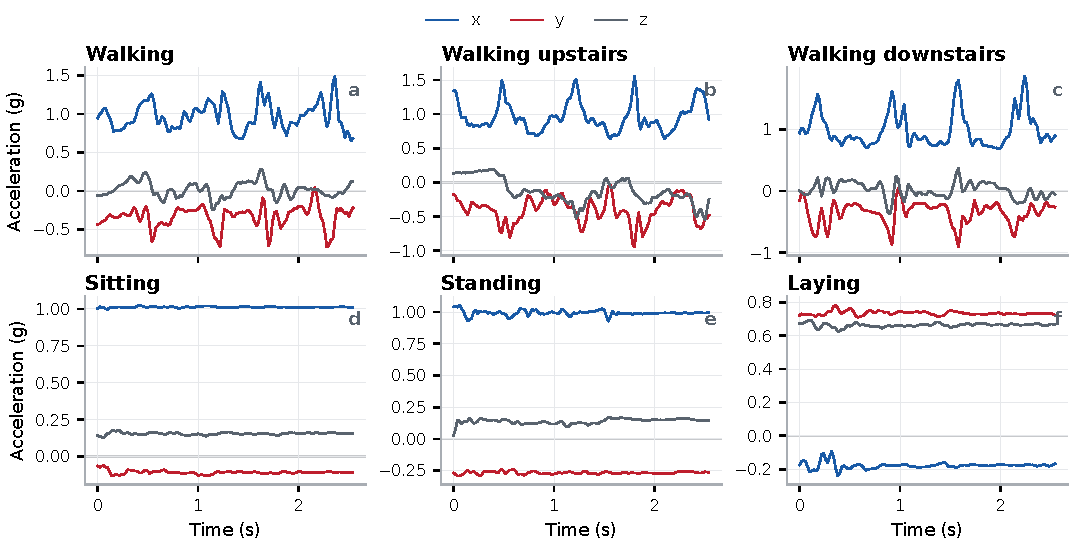
\includegraphics[width=\textwidth]{raw_signal_examples.pdf}
    \end{column}
    \begin{column}{0.33\textwidth}
      \small
      \vspace{0.10cm}
      \textbf{Motion versus stillness:} one energy or variance feature can be enough.
      \vspace{0.18cm}

      \textbf{Six activities}
      \begin{itemize}
        \item Posture changes the gravity projection.
        \item Walking patterns are periodic and multi-axis.
        \item Stair direction is a subtle within-motion distinction.
      \end{itemize}
      \vspace{0.08cm}
      \takeaway{A valid test can observe the wrong thing.}
    \end{column}
  \end{columns}
  \slidesource{UCI HAR held-out windows; Anguita et al., 2013}
\end{frame}

\begin{frame}{The classifier is a six-hypothesis GLRT}
  \small
  \setlength{\abovedisplayskip}{4pt}
  \setlength{\belowdisplayskip}{4pt}
  \begin{columns}[T,onlytextwidth]
    \begin{column}{0.53\textwidth}
      \vspace{0.08cm}
      For each activity $k$,
      \[
        \mathcal H_k:x\sim\mathcal N(\mu_k,\Sigma_k).
      \]
      Fit $(\widehat\mu_k,\widehat\Sigma_k)$ using training subjects, then score
      \[
        \ell_k(x)=-\tfrac12\!\left[
        \log|\widehat\Sigma_k|+(x-\widehat\mu_k)^\top
        \widehat\Sigma_k^{-1}(x-\widehat\mu_k)\right].
      \]
      \[
        \widehat y=\arg\max_k\ell_k(x),\qquad
        G=2(\ell_{1}-\ell_{2}).
      \]
      \vspace{0.10cm}
      {\color{SignatureBlue}\textbf{$G$ compares winner and runner-up evidence.}}\\[0.10cm]
      {\color{SignatureDark}\tiny Kay, \emph{Detection Theory}, 1998; Friedman, JASA, 1989}
    \end{column}
    \begin{column}{0.43\textwidth}
      \textbf{15 original features}
      \begin{itemize}
        \item axis means and log variances
        \item cross-axis correlations
        \item jerk energy
        \item dominant frequency, entropy, band power
      \end{itemize}
      \vspace{0.14cm}
      \textbf{9 WISDM additions}
      \begin{itemize}
        \item gravity-parallel and horizontal motion
        \item magnitude, jerk, and spectral summaries
      \end{itemize}
    \end{column}
  \end{columns}
\end{frame}

\begin{frame}{Testing is separated by person}
  \begin{columns}[T,onlytextwidth]
    \begin{column}{0.52\textwidth}
      \vspace{0.18cm}
      \begin{tabular}{lrrrr}
        \toprule
        Dataset & Hz & Window & Train & Test \\
        \midrule
        UCI HAR & 50 & 128 & 7,352 & 2,947 \\
        WISDM & 20 & 200 & 3,597 & 1,628 \\
        \bottomrule
      \end{tabular}
      \vspace{0.30cm}
      \begin{itemize}
        \item UCI HAR: 21 training, 9 test subjects
        \item WISDM: 24 training, 12 test subjects
        \item No test person enters scaling, fitting, or model selection
      \end{itemize}
    \end{column}
    \begin{column}{0.43\textwidth}
      \textbf{Training-only comparisons}
      \begin{enumerate}
        \item scalar variance baseline
        \item 15D Gaussian GLRT
        \item heavy-tailed Student-$t$ GLRT
        \item gravity-aligned features with two-parameter RDA
      \end{enumerate}
      \vspace{0.22cm}
      \textbf{Selection objective}\par
      Balanced accuracy across subject folds
      \vspace{0.22cm}
      \takeaway{The unit of generalization is a new person.}
    \end{column}
  \end{columns}
  \slidesource{UCI HAR DOI 10.24432/C54S4K; Kwapisz et al., 2011}
\end{frame}

\begin{frame}{Representation matters more than heavier tails}
  \centering
  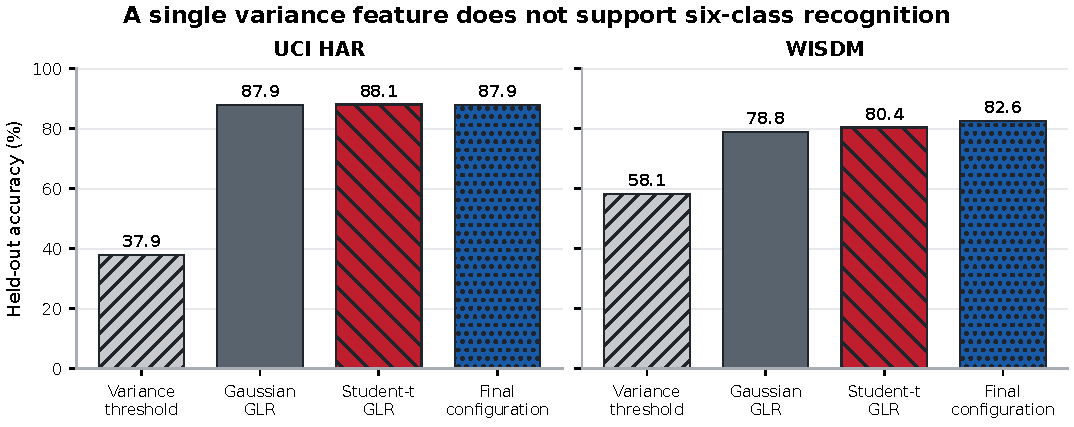
\includegraphics[width=0.86\textwidth]{performance_overview.pdf}
  \vspace{-0.05cm}

  \takeaway{Gravity alignment helps WISDM; the original 15D model remains the UCI choice.}
\end{frame}

\begin{frame}{The remaining errors are structured}
  \centering
  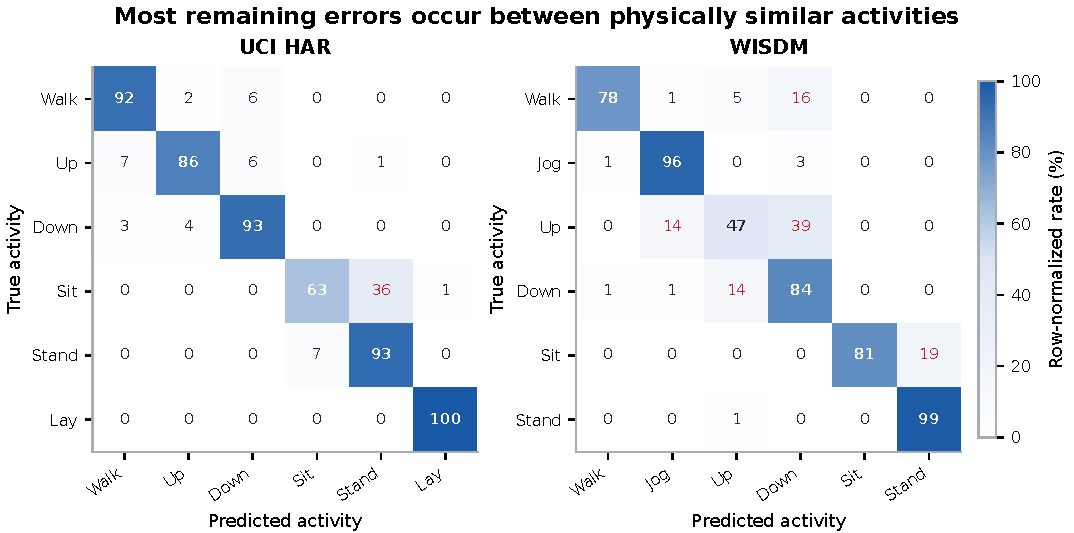
\includegraphics[width=0.76\textwidth]{confusion_matrices.pdf}
  \vspace{-0.10cm}

  \begin{columns}[T,onlytextwidth]
    \begin{column}{0.48\textwidth}
      \small
      \textbf{UCI HAR:} sitting is often called standing; laying is distinct.
    \end{column}
    \begin{column}{0.48\textwidth}
      \small
      \textbf{WISDM:} upstairs is confused with downstairs and jogging.
    \end{column}
  \end{columns}
\end{frame}

\begin{frame}{Average improvement hides subject variation}
  \begin{columns}[T,onlytextwidth]
    \begin{column}{0.72\textwidth}
      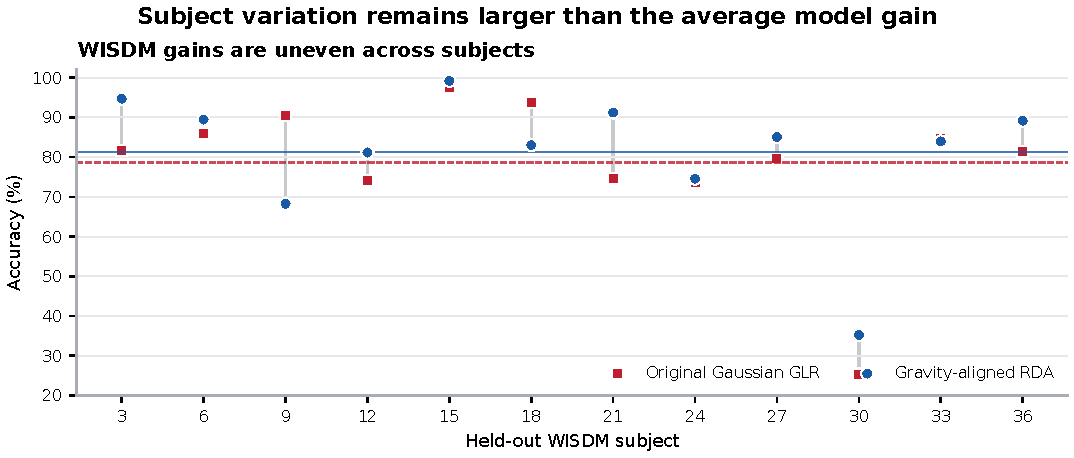
\includegraphics[width=\textwidth]{subject_variation.pdf}
    \end{column}
    \begin{column}{0.25\textwidth}
      \vspace{0.28cm}
      WISDM improves by 3.8 percentage points on average.
      \vspace{0.28cm}

      Several people gain strongly. Some regress. One remains near chance for both models.
      \vspace{0.28cm}

      \takeaway{A new cohort is still the hard case.}
    \end{column}
  \end{columns}
\end{frame}

\begin{frame}{The GLR margin can support a reject option}
  \begin{columns}[T,onlytextwidth]
    \begin{column}{0.60\textwidth}
      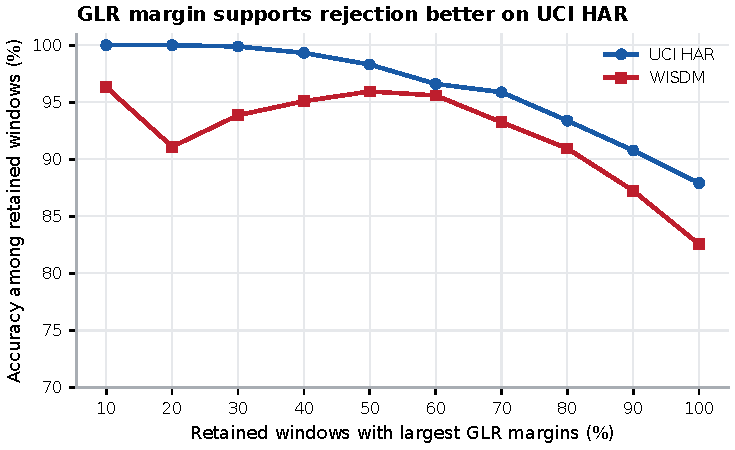
\includegraphics[width=\textwidth]{confidence_coverage.pdf}
    \end{column}
    \begin{column}{0.36\textwidth}
      \vspace{0.32cm}
      Sorting windows by $G$ concentrates correct predictions near the top.
      \vspace{0.28cm}

      At 50\% coverage:
      \begin{itemize}
        \item UCI HAR: 98.0\% correct
        \item WISDM: 96.0\% correct
      \end{itemize}
      \vspace{0.18cm}
      $G$ is not a calibrated probability. A deployment threshold needs independent validation.
    \end{column}
  \end{columns}
\end{frame}

\begin{frame}{What we learned and what comes next}
  \begin{columns}[T,onlytextwidth]
    \begin{column}{0.48\textwidth}
      \textbf{Evidence from this study}
      \begin{itemize}
        \item Six-class GLRT: 87.9\% on UCI HAR, 82.6\% on WISDM.
        \item Heavy tails help less than a better coordinate system.
        \item UCI posture and WISDM stair direction need different fixes.
        \item One configuration should not be forced across datasets.
      \end{itemize}
    \end{column}
    \begin{column}{0.48\textwidth}
      \textbf{Next experiments}
      \begin{itemize}
        \item evaluate a genuinely continuous, transition-annotated stream
        \item add gyroscope and direction-preserving body-frame features
        \item calibrate rejection on unseen subjects
        \item confirm on a new subject cohort
      \end{itemize}
    \end{column}
  \end{columns}
  \vfill
  {\color{SignatureBlue}\rule{\textwidth}{1.2pt}}\\[0.18cm]
  {\small Code, predictions, and figure scripts:}\\[0.05cm]
  {\color{SignatureBlue}\small\url{github.com/Harizz076/smartphone-har-activity-change-detection}}
\end{frame}

\end{document}
